%% LaTeX2e Template by Stephen Iota (https://stepheniota.com/)
%% last updated: Feb. 2019
%% for papers
%\documentclass[aps,preprint,notitlepage]{revtex4-1}
%% https://www-d0.fnal.gov/Run2Physics/WWW/templates/revtex4.pdf
%% https://cdn.journals.aps.org/files/revtex/auguide4-1.pdf
%% ^^ revTeX4-1 class options

%% for other
\documentclass[11pt]{article}
\usepackage{geometry} % let's be honest, standard LaTeX margins are GaRbagE for most purposes
%%%%%%%%%%%%%%%%
%%% Packages %%%
%%%%%%%%%%%%%%%%

\usepackage[utf8]{inputenc}
\usepackage[noadjust]{cite}
%\usepackage{lipsum}
\usepackage{amsmath}
\usepackage{amssymb}
\usepackage{amsfonts}
\usepackage{physics} %http://ftp.math.purdue.edu/mirrors/ctan.org/macros/latex/contrib/physics/physics.pdf
\usepackage[thinc]{esdiff} % easy derivatives
\usepackage{graphicx} % \includegraphics{ }
\usepackage[shortlabels]{enumitem} % change labels in enum/item environments
\usepackage[dvipsnames]{xcolor} % colored links=
%\usepackage{footmisc} % http://mirror.utexas.edu/ctan/macros/latex/contrib/footmisc/footmisc.pdf
%\usepackage[small]{titlesec} % [small,medium,big] << controls size of *section text
%\usepackage{fancyhdr} %http://tug.ctan.org/tex-archive/macros/latex/contrib/fancyhdr/fancyhdr.pdf
% always put this at the end
\usepackage[
	colorlinks=true,
	citecolor=NavyBlue!90!black,
	linkcolor=NavyBlue!75!black,
	urlcolor=green!50!black,
	hypertexnames=false]{hyperref}

 %%%%%%%%%%%%%%%%%%
 %% New Commands %%
 %%%%%%%%%%%%%%%%%%
\newcommand{\email}[1]{\texttt{\href{mailto:#1}{#1}}}


%%%%%%%%%%%%%%%%%%
%% Front Matter %%
%%%%%%%%%%%%%%%%%%

%\pagenumbering{gobble} % no page numbers
\graphicspath{{figures/}} % set directory for figures
%\setcounter{section}{-1} % start with section 0


%%%%%%%%%%%%%
%%% Title %%%
%%%%%%%%%%%%%
\begin{document}

\begin{center}

\Large{\textsc{PSet 4}: \textbf{Traveling Waves}}
\end{center}
\vspace{.5mm}


%%%%%%%%%%
%% INFO %%
%%%%%%%%%%

\begin{tabular}{rl}
\textsc{SI Leader}:
&
Stephen Iota (\email{siota001@ucr.edu})
\\
\textsc{Course}:
&
Physics 40B (Spring 2019), Prof.~Barsukov
\\
\textsc{Date}:
&
\today
\end{tabular}

%%%%%%%%%%%%%%
%% PROBLEMS %%
%%%%%%%%%%%%%%

\section{The wave model}
\begin{enumerate}[(a)]
	\item What is a traveling wave?
	\item What is the main requirement in order for a traveling wave to propagate?
	\item Describe the difference between a transverse and a longitudinal wave.
	\item How do we define a wave's velocity? What does it depend upon?
	\item Is wavelength of a wave a property of the medium or the source? What about frequency? Explain.
\end{enumerate}

\section{History and snapshop graphs}

\begin{enumerate}[(a)]

\item Below is a snapshot graph at $t = 0$ sec for a wave moving to the right at a speed of 2.0 m/s. Draw a history graph for the position $x = 8.0$ m.
\begin{center}
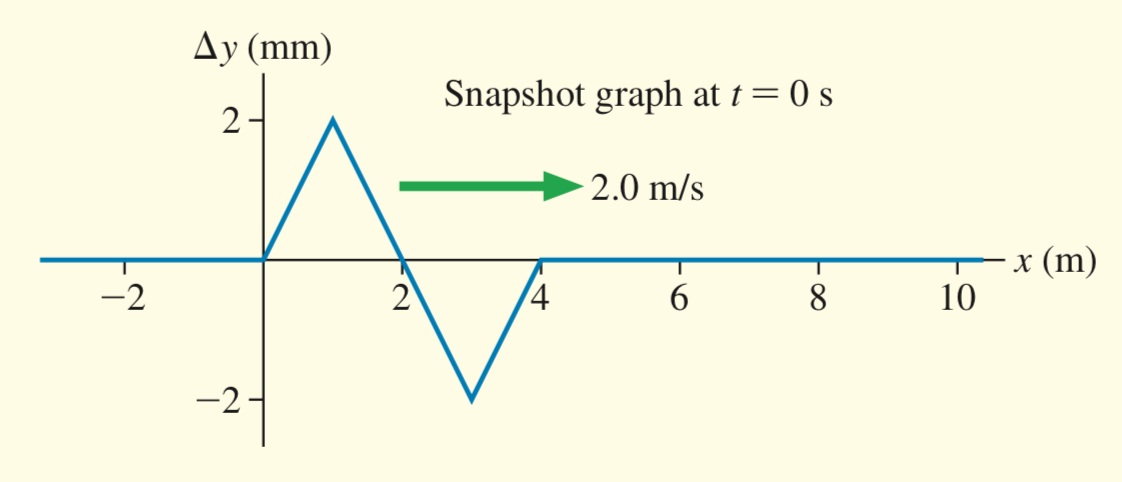
\includegraphics[width=.5\linewidth]{PSet4_FigA}
\end{center}

\item What is the frequency of the traveling wave below?
\begin{center}
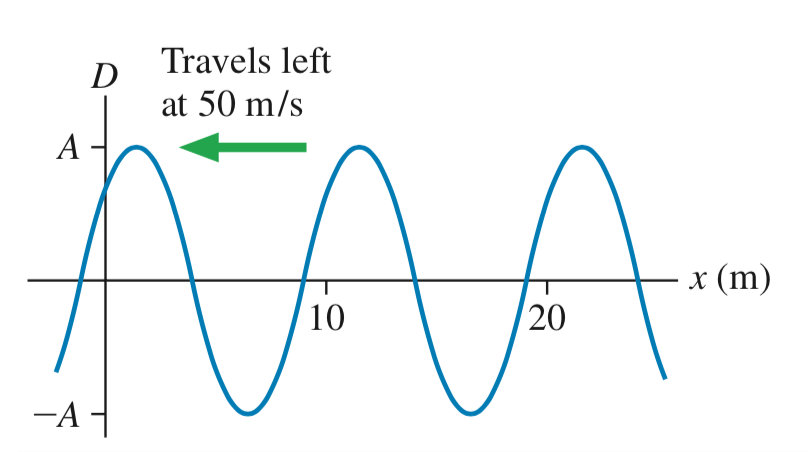
\includegraphics[width=.5\linewidth]{PSet4_FigB}
\end{center}


\item Draw the history graph $D(x = 0 \ \text{m},t)$ for the wave shown below.
\begin{center}
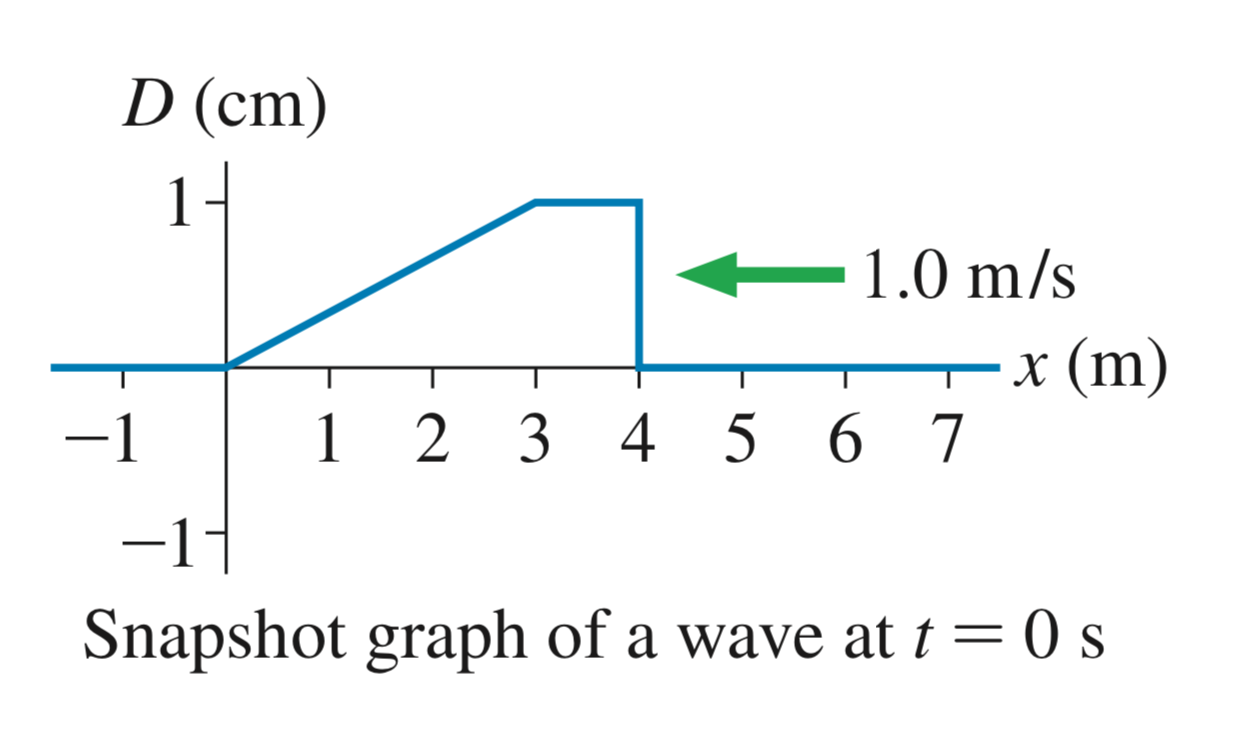
\includegraphics[width=.5\linewidth]{PSet4_FigC}
\end{center}

\end{enumerate}


\section{Sinusoidal traveling waves}
A very long string with $\mu = 2.0$ g/m is streched along the $x$-axis with a tension of 5.0 N. At $x=0$ m, it is tied to a 100 Hz simple harmonic oscillator that vibrates perpendicular to the string with an amplitude of 2.0 mm. The oscillator is at maximum displacement initially.

\begin{enumerate}[(a)]
	\item Write the displacement equation for the traveling wave on a string

	\item At $t = 5.0$ ms, what is the string's displacement at a point 2.7 m from the oscillator?
\end{enumerate}



\end{document}
